\chapter{Supplementary Material for \cref{alevin}}
\label{appendix-alevin}

\section{ Machine Configuration and Pipeline Replicability }
\label{sec:tool_params}

%10x v1 chemistry benchmarking has been scripted using Snakemake \cite{snakemake} and performed on an Intel(R) Xeon(R) CPU (E5-2699 v4 @2.20GHz with 44 cores and 56MB L3 cache) with 512GB RAM and a 4TB TOSHIBA MG03ACA4 ATA HDD running Ubuntu 16.10.

10x v2 chemistry benchmarking has been scripted using CGATCore (https://github.com/cgat-developers/cgat-core). The full pipeline and analysis are performed using Stony Brook's seawulf cluster with 164 Intel Xeon E5-2683v3 CPUs.

For all analyses, the genome and gtf versions used for human datasets was GENCODE release 27, GRCh38.p10 and for mouse datasets was GENCODE release M16, GRCm38.p5. All transcriptome files were generated using these with ``rsem-prepare-reference".

\textbf{\cellr (v2.2.0):} The following additional flags were used, as recommended by the \cellr guidelines: \texttt{--nosecondary --expect-cells NumCells}, where NumCells is 10,000 for PBMC 8k and Neurons 9k,
5,000 for PBMC 4k, 2,000 for Neurons 2k and Neurons 900.

\textbf{\Alevin (v0.13.0):} Run with default parameters with the chromium protocol and \texttt{--keepDuplicates} flags and the \texttt{-lISR} to specify strandedness. The mRNA and rRNA lists were obtained from the relevant annotation files and passed as input. Experiments on v1 chemistry can be run using the same flags but with the \texttt{--gemcode} protocol flag.  \Alevin also supports 10x v3 chemistry via the command-line flag \texttt{--chromiumV3}.

\textbf{STAR (v2.6.0a):} The following flag was used, as recommended by the guidelines of UMI-tools: \\ \texttt{--outFilterMultimapNmax 1} 

\textbf{featureCounts (v1.6.3):} This was run to obtain an output BAM file and with stranded input (\texttt{-s 1}).

\textbf{UMI-tools (v0.5.4):} The extract command was used to get the CBs/UMIs, when provided with an external CB whitelist, and attach it to the corresponding reads. The following flags were used in the count command to obtain the per cell gene count matrix: \texttt{--gene-tag=XT --wide-format-cell-counts}

\dropest (v0.8.5): This was run with the default parameters on the 10x BAM files and the predicted cell counts from \cellr were used as input.

\textbf{Dropseq utils (v2.0.0):} All the commands were run as recommended by the authors in the tool's manual.

The bulk datasets were quantified using Bowtie2 and RSEM, run as follows:

\textbf{Bowtie2 (v2.3.4.3):} The following flags were used, as recommended in the guidelines of RSEM: \texttt{--sensitive --dpad 0 --gbar 99999999 --mp 1,1 --np 1 --score-min L,0,-0.1 --no-mixed \\ --no-discordant}

\textbf{RSEM (v1.3.1):} Run with default parameters.


%%%%%%%%%%%%%%%%%%%%%%%%%%%%%%%%%%%%%%%%%%%%%%
%%                                          %%
%% Backmatter begins here                   %%
%%                                          %%
%%%%%%%%%%%%%%%%%%%%%%%%%%%%%%%%%%%%%%%%%%%%%%

\section{Availability of data and materials}
\Alevin is implemented in \texttt{C++14} and is released under the GNU General Public License v3.0. The source code as used in the chapter has been deposited in archived format at \url{https://doi.org/10.5281/zenodo.2583275}~\citep{scode} and the latest code is available at \url{https://github.com/COMBINE-lab/salmon}~\citep{alvgit}. The output quantification results of all the tools used in the validation of \alevin-pipeline have been deposited in archived format at \url{https://doi.org/10.5281/zenodo.2583228}~\citep{vdata}.

All the single cell 10x datasets used in the chapter are taken from \url{https://support.10xgenomics.com/single-cell-gene-expression/datasets}~\citep{v2data} and the DropSeq data is from SRR1853180. The relevant accessions for the bulk RNA-seq datasets used for the validation are listed in~\Cref{suptab:bulkmmRate}.

\newpage
\section{Additional Figures}
\begin{figure*}[!htb]
    \centering
  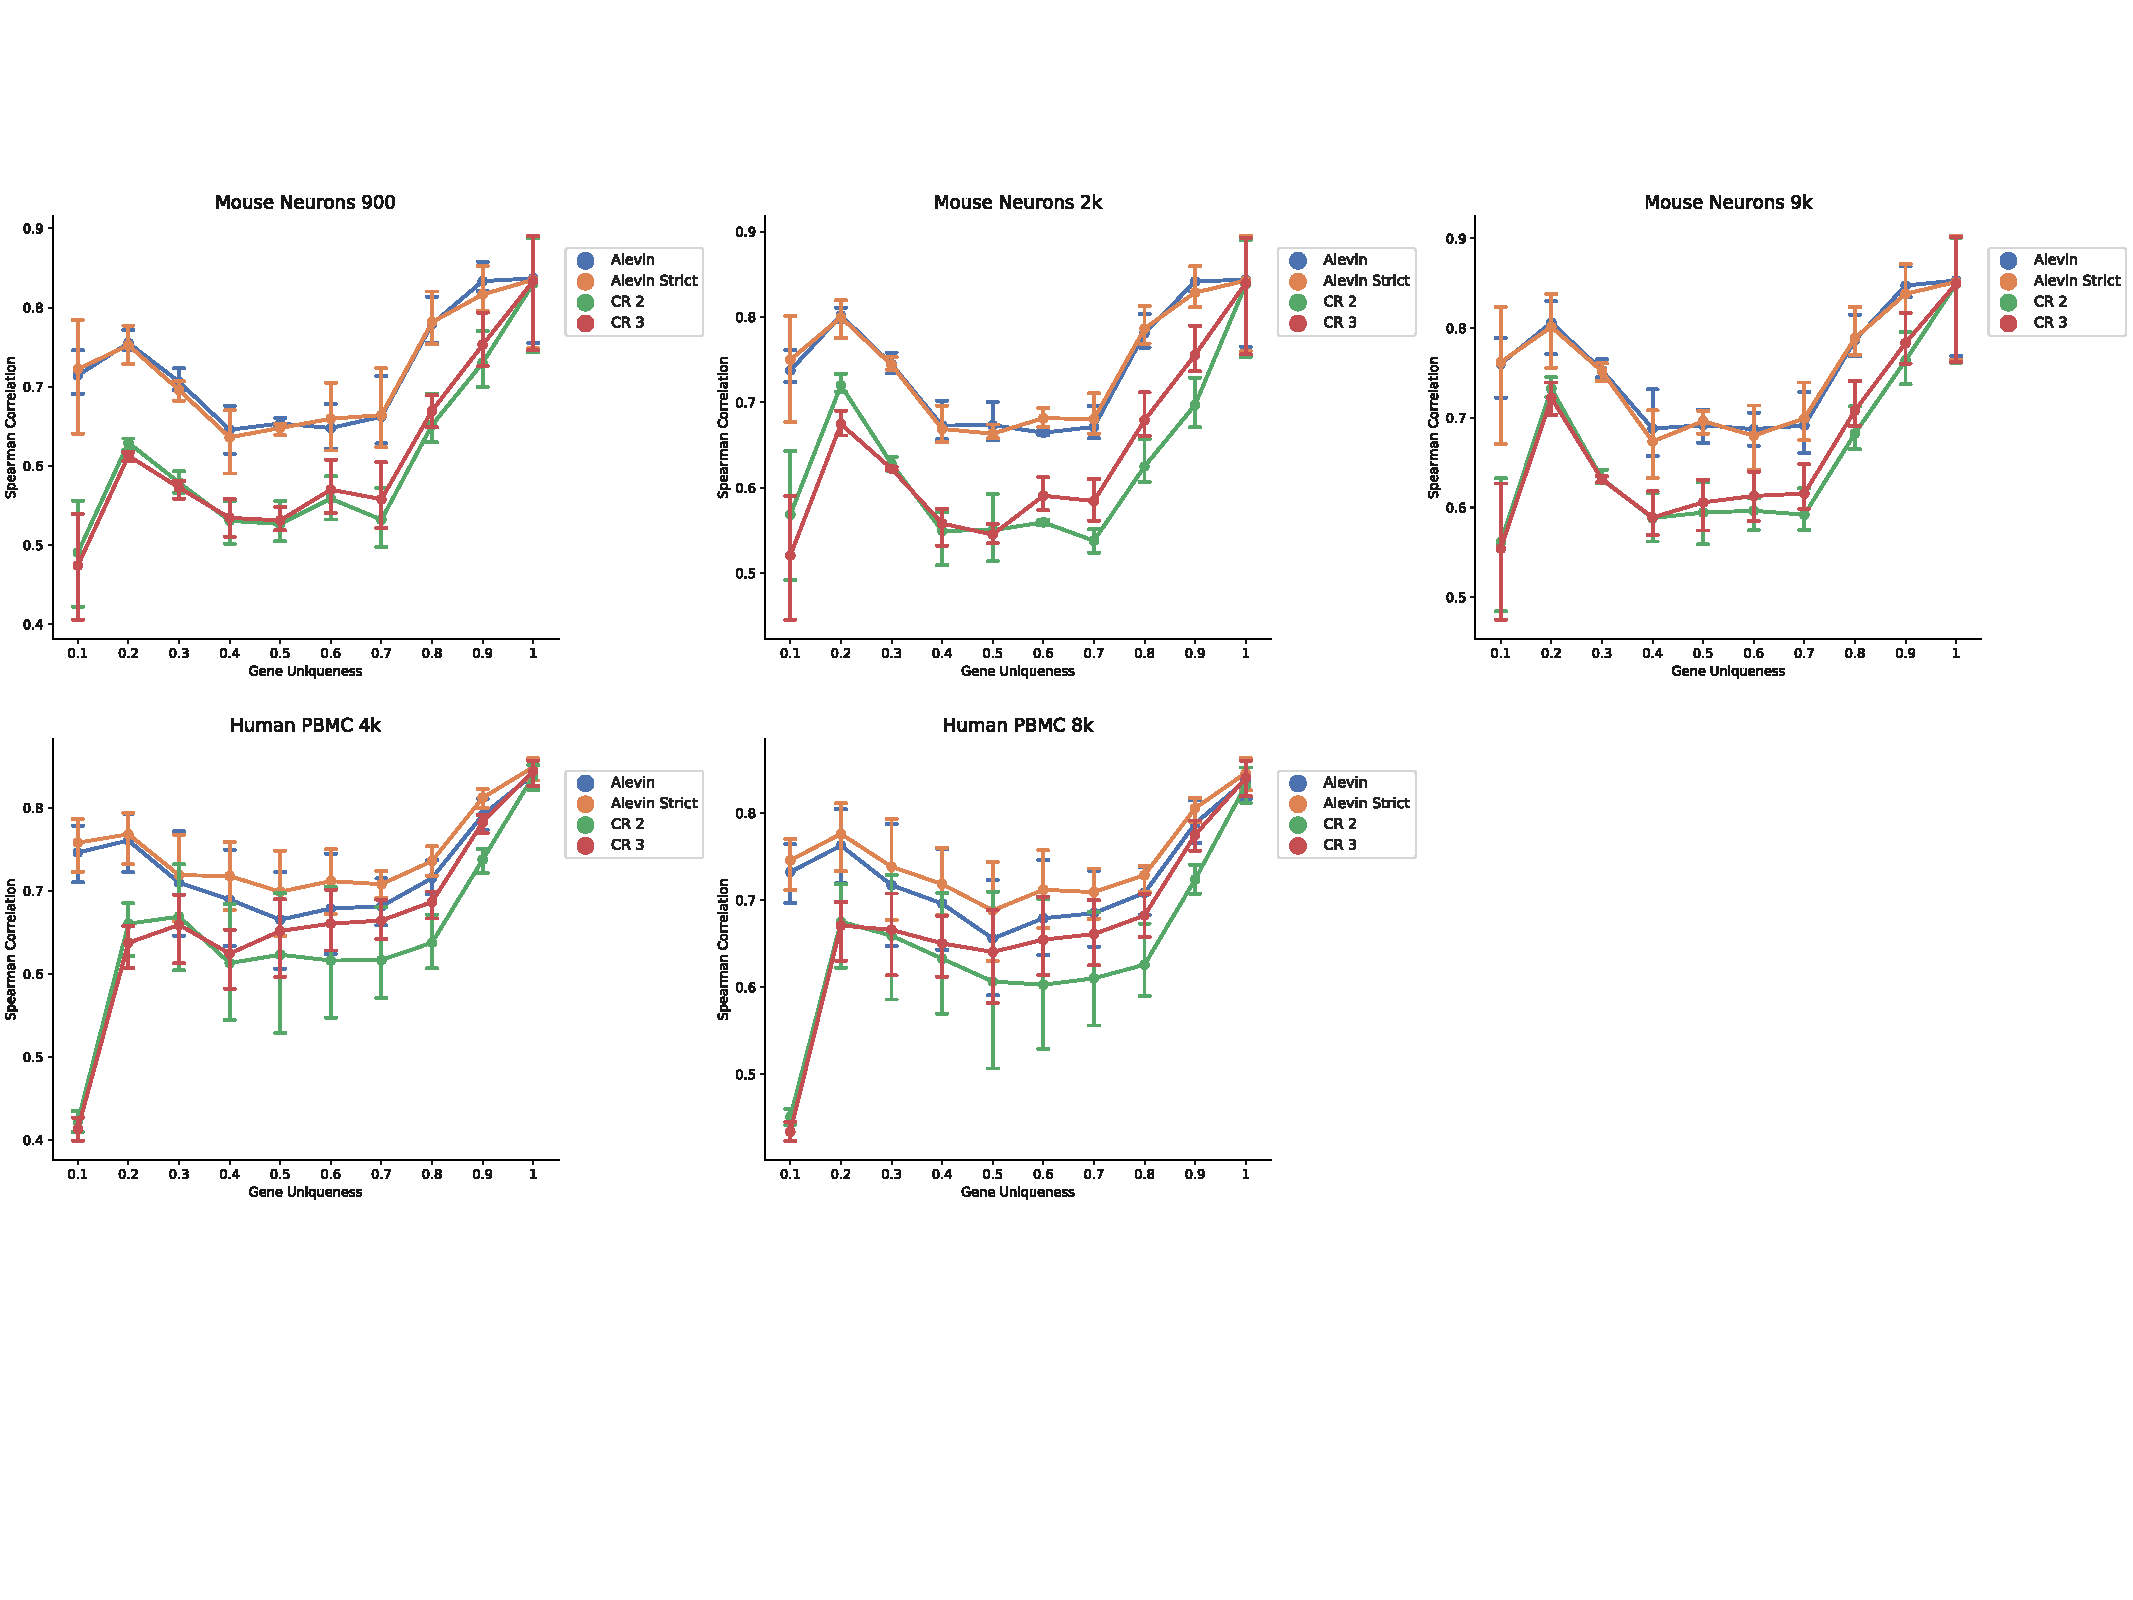
\includegraphics[width=\linewidth]{alevin/supp_combine_corr.pdf}
  \caption{The Spearman correlation between quantification estimates from different runs of \alevin and \cellr. Note that two different versions \cellr were run with the default parameters and \alevin strict refers to the same version of \alevin run with \texttt{--minScoreFraction} set to 0.95 and \texttt{--consensusSlack} set to 0.99. These parameters in \alevin make the mapping filter strict and allows fewer spurious mappings.}
  \label{suppfig1}
\end{figure*}

\begin{figure*}[!htb]
    \centering
  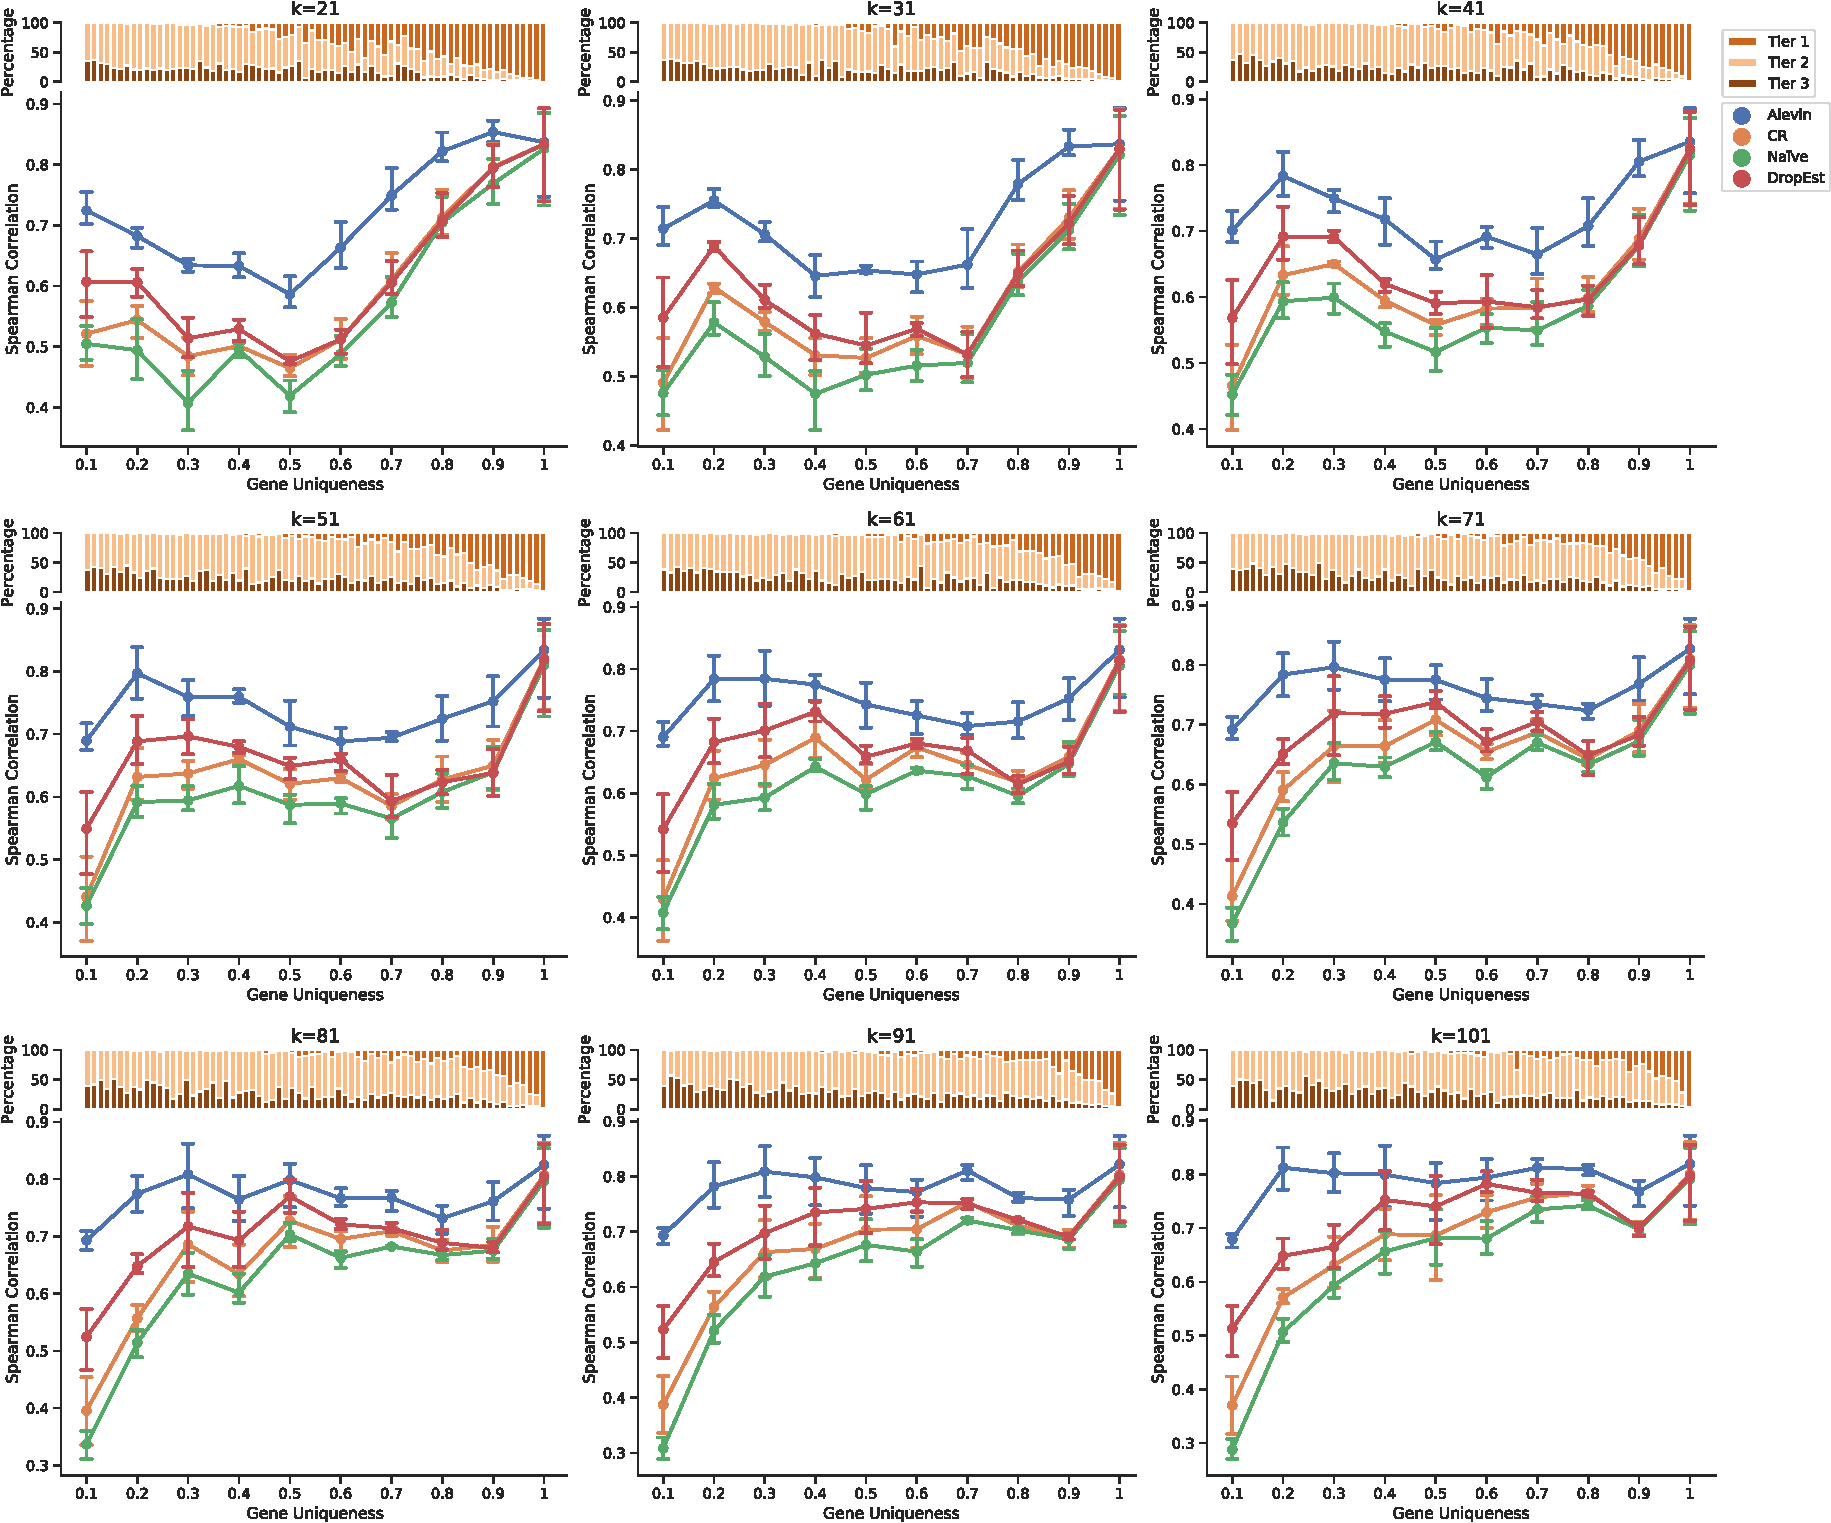
\includegraphics[width=\linewidth]{alevin/supp_combine_uniq.pdf}
  \caption{Correlation plots for the mouse neuronal 900 dataset using different values of the k-mer size (k) to calculate gene uniqueness.}
  \label{suppfig2}
\end{figure*}

\begin{figure*}[!htb]
    \centering
  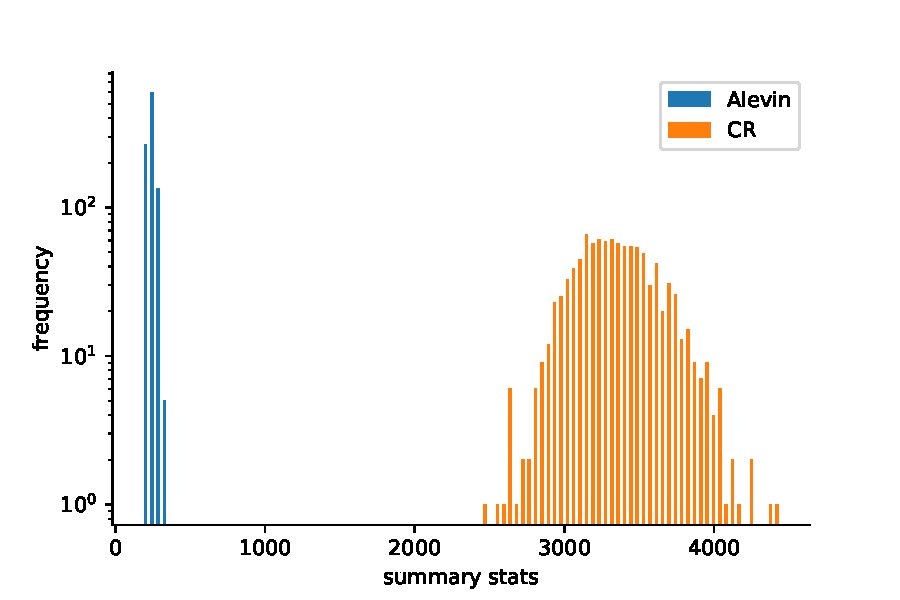
\includegraphics[width=0.8\linewidth]{alevin/supp_pvals.pdf}
  \caption{The histogram is the result of taking $1000$ samples of $100$
    cells each from the mouse neuronal 900 dataset, and looking at the sum of
    absolute differences when quantifying the data under the varying reference
    genomes (mouse vs. mouse and human combined).}
  \label{suppfig3}
\end{figure*}